%
%%%%%%%%%%%%%%%%%%%%%%%%%%%%%%%%%%%%%%%%%%%%%%%%%%%%%%%%%%
%
%  U M S E T Z U N G   &   I M P L E M E N T I E R U N G
%
%%%%%%%%%%%%%%%%%%%%%%%%%%%%%%%%%%%%%%%%%%%%%%%%%%%%%%%%%%
\chapter{Umsetzung \& Imlementierung}
\label{cha:umsetzung}
%
Nun kommen wir an den praktischen Teil der Arbeit. In diesem Kapitel wird zunächst einiges über die Entwicklungsumgebung gesagt. Anschließend wird auf wesentliche Punkte der Umsetzung und Implementierung eingegangen. Dabei wird wieder auf die Anforderungen zurückgegriffen und erläutert wie diese umgesetzt wurden. Vorraussetzung für dieses Kapitel ist das Grundlagenkaptitel der Arbeit, um zusammenhänge mit den Technologien besser verstehen zu können.
\section{Entwicklungsumgebung}
\label{sec:umsetzung}
%
Dieses Kapitel befasst sich mit den verwendeten Technologien, die eine produktive Entwicklung ermöglichen. Es wird auf alle verwendeten Technologien, Bibliotheken sowie Programme eingegangen und begründet, warum eine Verwendung sinnvoll ist.\\
\paragraph{Technologien und Bibloetheken}
Wie in den vergangenen Kapiteln schon erläutert sind die Haupttechnologien das Framework \textit{Angular} sowie die 3D Bibliothek \textit{Three.js}, welche WebGL zum Einsatz bringt. Angular Anwendungen werden grundsätzlich mit \textit{Node.js} installiert. Dadurch ist es uns später möglich verschiedene npm-Module wie Three.js oder auch Bootstrap zu installieren. Zusätzlich nutzt Angular \textit{Webpack}, um den Quellcode zu bündeln. Dabei werden die scss-Dateien in eine css-Datei komprimiert. Sass in Verbindung mit \textit{Webpack} ist nicht nur in für Angular-Projekte ein beliebtes Tool zum entwickeln von Webseiten und Webanwendungen. Auch eine Versionierung des Quellcodes kommt zum Einsatz. Mit \textit{Git} ist der Quellcode immer gesichert und man kann nach dem Testen einer bestimmten Funktion immer wieder zum letzten Push zurückkehren. Bei einem Bachlor-Projekt kann man zwar nicht den Vorteil der Teamentwicklung mit \textit{Git} nutzen, jedoch kann man damit sehrwohl seinen Quellcode versionieren und sichern, was bei einem Bachlorprojekt durchaus sinnvoll erscheint. 
\paragraph{Entwicklungswerkzeuge} Als Text-Editor wird \textit{PhpStorm} verwendet. Dadurch ist eine flexible Programmierung an unterschiedlichen Systemen möglich, da der Editor für Windows, MacOS als auch für Linux verfügbar ist. Er bietet eine praktische Integration von Git und kann dazu noch sehr gut mit Angular-Anwendungen arbeiten. Auch Angular CLI Befehle können teilweise direkt in dem Editor ausgeführt werden und \textit{PhpStorm} verfügt über eine logische Code-Verfolständigung. Nicht zu vergessen die optimale Quellcode-Formatierung für jeden Dateityp. \textit{PhpStorm} verfügt zwar über ein integriertes Terminal, jedoch ist das meist sehr unpraktisch, da es nur unnötig Platz in der Anwendung wegnimmt. Deswegen werden Kommandozeilen einem zusätzlichen Terminal ausgeführt. Gerade am Anfang des Projekts wird die Angular CLI viel zum Einsatz kommen.
%
\section{Anlegen des Angular-Projekts}
\label{sec:umsetzung}
%
Bevor die Angular-Anwendung nach und nach aufgebaut werden kann, muss Angular erst einmal installiert werden und anschließend ein Projekt erstellt werden. Mit der Angular CLI ist das sehr einfach und unproblematisch. Deshalb ist der erste Schritt diese über Node.js zu installieren.
%
\section{Module des Konfigurators}
\label{sec:umsetzung}
%
Im folgenden Kapitel wird betrachtet aus welchen Module die Angular Anwendung aufgebaut ist. Anschließend werden die Module angelegt. Es geht hier nur um das Anlegen der Module, noch nicht um die Funktionalität der einzelnen Module. Die Abbildung zeigt eine Übersicht aller Module, welche in der Webanwendung implementiert sind\footnote{Hierbei ist zu beachten, dass die Abbildung auf die wesentlichen Module beschränkt ist, da es sonst zu unübersichtlich werden würde. Eine vollständige Übersicht der Module befindet sich im Anhang.}.
\begin{figure}[h]
	\centering
	{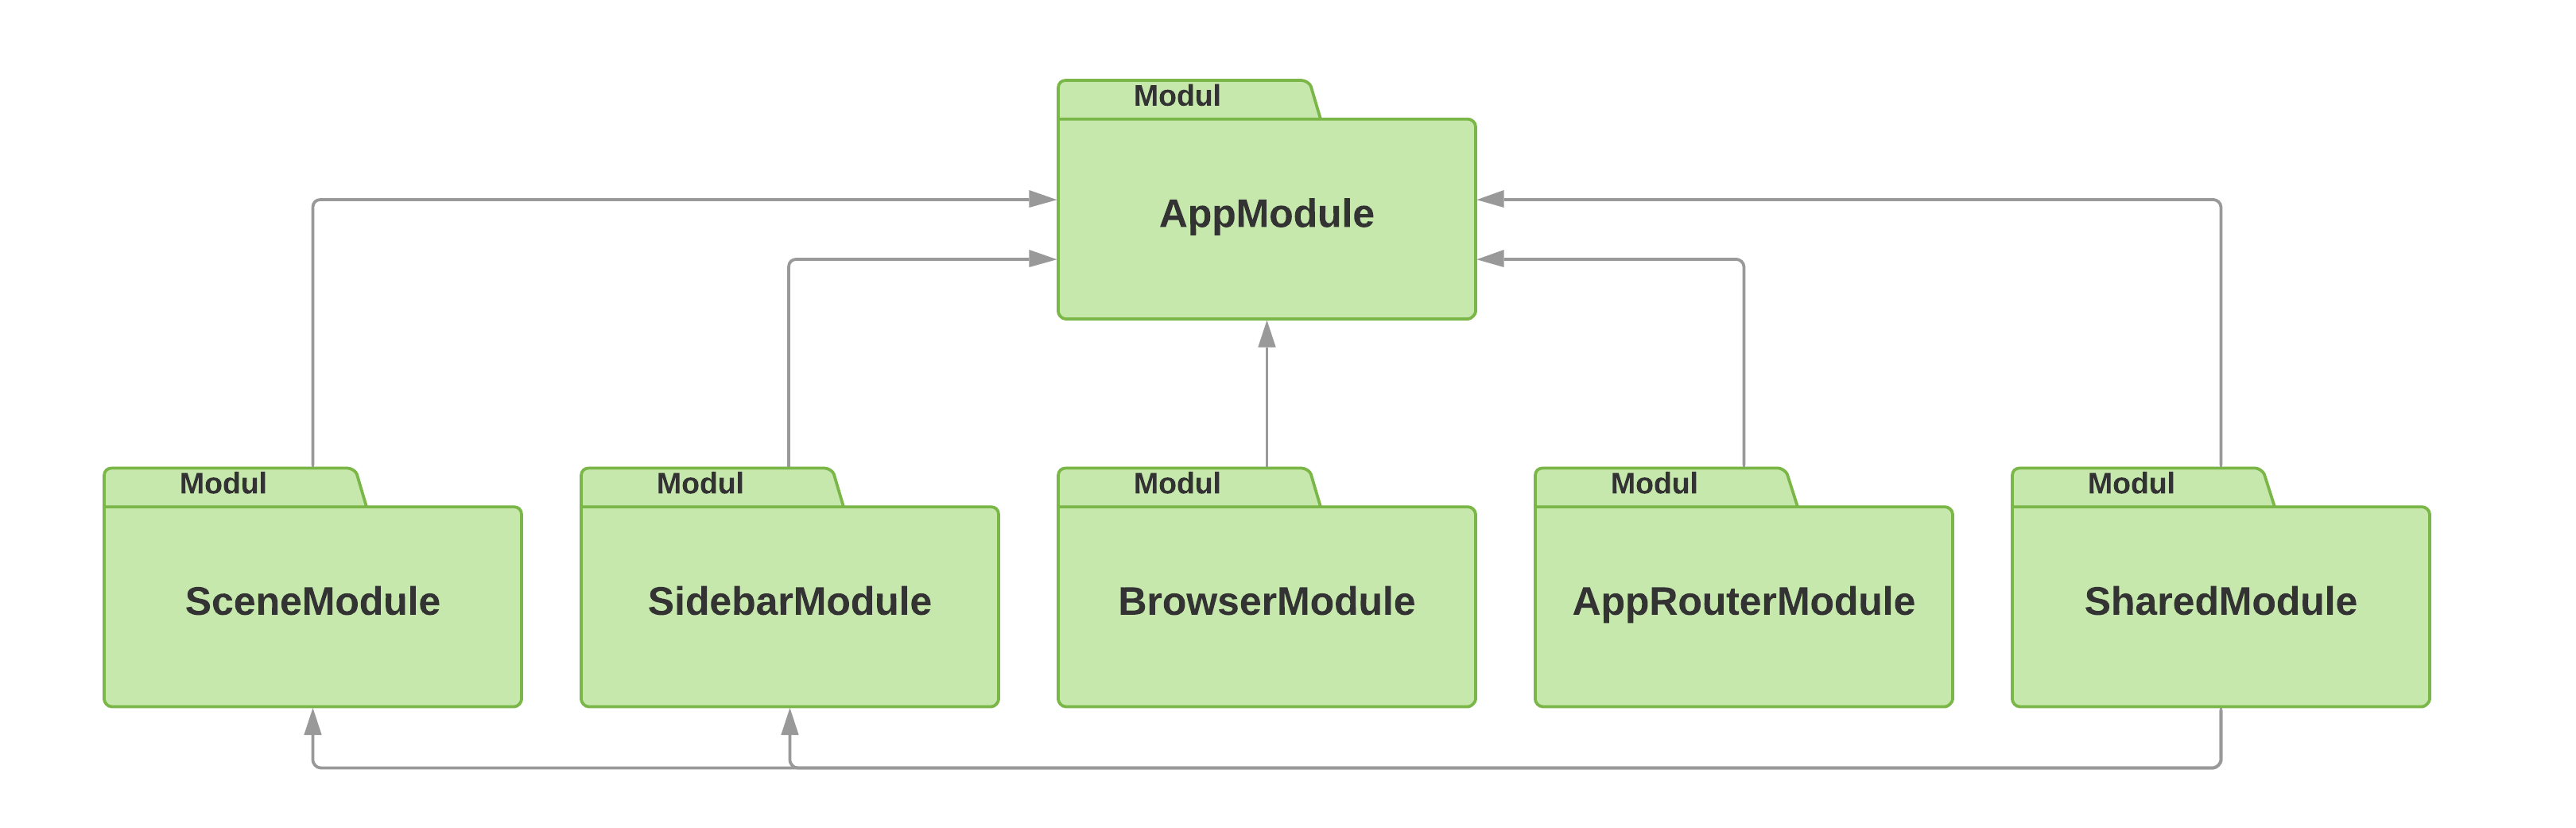
\epsfig{file = umsetzung/images/module.png, width=13.0cm}}
	\caption[Übersicht der Module]{\textit{Module der Angular-Anwendung}}
	\label{fig:module}
\end{figure}
Die einzelnen Bausteine der Angular-Anwendung werden im Rahmen dieses Bachlorprojektes immer über die Angular CLI generiert, da das am einfachsten funktioniert und zeitsparend ist. Ein Modul kann mit folgendem Command Line Befehl generiert werden:
%
\begin{lstlisting}
ng g m shared
\end{lstlisting}
%
Als Beispiel wurde hier das Module \textit{shared} angelegt. Hierin werden später alle globalen Bausteine der Angular-Anwendung erstellt. Es wurden außerdem die Appkürzungen \texttt{m} für \texttt{module} und \texttt{g} für \texttt{generate} verwendet. Ob ausgeschrieben oder abgekürzt, das hat keine Auswirkungen, sondern spart lediglich Zeit. Es gibt noch ein paar Zusatzoptionen, die als Parameter angegben werden können. Diese sind in der offizielen Dokumentation von Angular aufgeführt. Diese ermöglichen verschiedene Funktionen wie \texttt{export}-Funktion oder verhindern das generieren von Testdateien. Der 3D Konfigurator hat noch zwei weitere wichtige Module. Zum einen ist das \textit{SceneModule} für die 3D Darstellung zuständig und das Rendern des Designs. Das \textit{SidebarModule} ist sozusagen das Konfigurationsmenu inklusive einer Übersicht in tabellarischer Form. Die hauseigenen Module von Angular wie das \textit{BrowserModule} wurden von der Angular CLI automatisch importiert. Hier ist also kein weiterer Schritt notwendig, die Anwendung sollte lauffährig sein. Noch hat die Applikation allerdings noch keine richtige Funktionalität.
%
\section{Komponenten des Konfigurators}
\label{sec:umsetzung}
%
Sowohl das \textit{SidebarModule} als auch das \textit{SceneModulue} des Konfigurators haben sozusagen eine \glqq Hauptkomponente\grqq. Diese werden dann später in der \textit{AppComponent} eingebunden. Die Basis-Komponente der Anwendung ist also sehr einfach und übersichtlich. Dann gibt es noch einige weitere Kindskomponenten sowie geteilte Komponenten (aus dem \textit{sharedModule}). In diesem Kapitel werden wir uns zunächst auf die Komponenten beschränken. Alle weiteren Bausteine wie Services werden wir später noch genauer betrachten.\\
Die \textit{SceneComponent} ist dafür da die komplette 3D-Szene zu erzeugen und eben das Becher-Model mit seinem Design darstellen soll. Wie alle Kompoentente wurde diese mittels Angular CLI in PhpStorm angelegt, wie in Abbildung \ref{fig:phpstorm} zu sehen. 
%
\begin{figure}[h]
	\centering
	\subfigure[Auswahl generierbarer Angular-Bausteine]{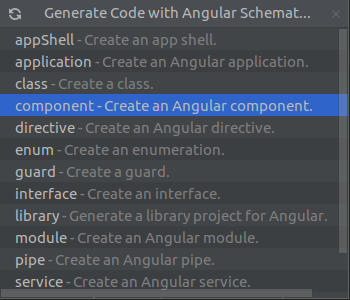
\includegraphics[width=5cm\textwidth]{umsetzung/images/auswahlcli.png}}
	\subfigure[Gernerieren einer Komponente mit Parametern]{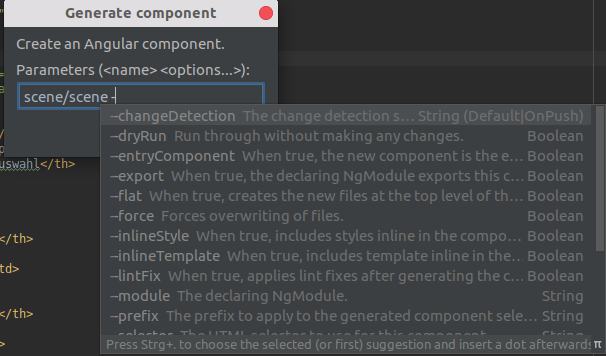
\includegraphics[width=7cm\textwidth]{umsetzung/images/optionscli.png}}\\	\subfigure[Generierte Dateien durch die CLI]{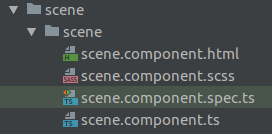
\includegraphics[width=5cm\textwidth]{umsetzung/images/generatedfiles.png}}
	\caption{\textit{Erstellung einer Angular-Komponente mit PhpStorm}}
	\label{fig:phpstorm}
\end{figure}
%
In PhpStorm kann man über \lstinline{File > New > Angular Schematics} innerhalb des Editors die Angular CLI verwenden. Wie im ersten Bild zu sehen, lassen sich so alle Bausteine von Angular anlegen. In diesem Fall wird eine Komponente angelegt. Nach der Auswahl wird man nun aufgefordert den Komponenten-Namen sowie optionale Parameter mit anzugeben. Das praktische ist, das PhpStorm alle verfügbaren Parameter vorschlägt und man nicht etwa in der Documentation nachschauen müsste, welchen Parameter man braucht und vermeidet Tippfehler. Nach bestätigen der Eingabe werden nun wie in Bild c) zu sehen alle erforderlichen Dateien der Komponente generiert. Zusätzlich werden im Hintergrund eventuelle Import-Anweisungen sowie Export- Anweisungen und so weiter automatisch ergänzt. In unserem Fall wurden auch die Testdatei erzeugt, welche wir uns im nächsten Kapitel genauer anschauen wollen. Die anderen drei Dateien sind wie wir wissen für Logik, Styles und Templating zuständig. Analog zu dem Erstellen der Komponente in PhpStorm funktioniert das ganze auch in einem Terminal:
%
\begin{lstlisting}
ng g c scene/scene -m=scene
\end{lstlisting}
%
Sobald die Komponente angelegt ist, hat sich eigentliche keine Funktionalität. Das wird erst später mit der Logik und den Services implementiert. Für den Anfang reicht es, hier schonmal das \texttt{canvas}-Element anzulegen und ein paar Styles in der \texttt{scss}-Datei der Komponente anzulegen. Wer sich mit \texttt{scss} bzw. \texttt{sass} auskennt, kann hier die Schreibweise nutzen. Man kann aber auch normales \texttt{css} schreiben. Damit ist die \textit{SceneComponent} im Grunde schon fertig.
\paragraph{Kindskomponente}
Genauso wie die \textit{SceneComponent} wurde auch die \textit{SidebarComponent} angelegt. Sie stellt die komplette Sidebar im rechten Bereich dar, also das Konfigurationsmenü und die Übersicht. Diese Komponente ist etwas komplexer und hat noch ein paar Kindskomponenten. Die Sidebar ist mit der Bootstrap-Komponente \textit{Tabs}\footnote{https://getbootstrap.com/docs/4.0/components/navs/\#tabs} umgesetzt. Wir haben also im Menu zwei Tabs, Konfigurator und Übersicht. Diese Tabs sind als eigene Komponente in \textit{SharedModule} implementiert und können in unserer SidebarCompontent also Kindskomponente verwendet werden. Es ist sozusagen ein eigener Typ für \textit{Tabs} definiert. Die Umsetzung der Tab-Komponente wird nun genauer beleuchtet.\\

Die Tabs von Bootstrap sind in einem \texttt{<ul>}-Element implementiert, welcher sozusagen den Container darstellt. Die einzelnen Tabs sind dann \texttt{<li>}-Elemente und werden durch die Liste gebündelt. Am Ende entsteht folgendes Template für die Tabs-Komponente:
%
\begin{lstlisting}
<ul class="nav nav-tabs nav-fill">
	<li class="nav-item" *ngFor="let tab of tabs" (click)="selectTab(tab)">
		<a [class.active]="tab.active" class="nav-link nav-title" href="#">{{tab.title}}</a>
	</li>
</ul>
<ng-content></ng-content>
\end{lstlisting}
%
Die \texttt{<ul>}-Liste hat ein paar vordefinierte Bootstrap-Klassen, auf die hier nicht weiter eingegangen wird. Sobald ein Tab aktiv ist, soll der dazugehörige Inhalt angezeigt werden. Wie im Quellcode zu sehen gibt es nur ein \texttt{<li>}-Tag, was nicht heißt, das es nur einen Tab gibt. Die Komponente sollte eine beliebige Anzahl an Tabs haben können. Das ist in diesem Fall dynamisch realisiert. Mit der Direktive \texttt{*ngFor} wird geprüft, wie viele Tabs im Template erstellt wurden und gibt diese dann mithilfe der for-Schleife aus. Damit wird allerdings noch nicht der Inhalt des aktiven Tab angezeigt. Dazu wird noch die \texttt{selectTab()}-Funktion benötigt. Bei \texttt{onClick} wird diese ausgeführt und teilt der Komponente mit, welcher Tab aktiv ist. Anschließend wird der Content durch \texttt{<ng-content>} ausgegeben. Um nun die Tabs als Komponente zu verwenden brauchen wird noch ein Tab-Komponente. Die Tabs-Komponente definiert, wie die Navigation insgesamt aufgebaut ist und die Tab-Komponente beschreibt, wie die einzelnen Tabs aufgebaut sind. Im Grunde werden hier nur die Inhalte des Tabs in einem div ausgegben. Wie oben im Quellcode zu sehen greifen wir auf die Variable \texttt{tab.active} und \texttt{tab.title} zu. Diese sind in Tab definiert. In unserer Sidebar würde die Tabs folgendermaßen verwendet:
%
\begin{lstlisting}
<gc-tabs>
	<gc-tab [tabTitle]="'Konfigurator'">
		Content 1
	</gc-tab>
	<gc-tab [tabTitle]="'Overview'">
		Content 2
	</gc-tab>
</gc-tabs>
\end{lstlisting}
%
Es könnten nun noch beliebig viele \texttt{<gc-tab>}-Elemente hinzugefügt werden und sie würden auch als Tab angezeigt werden. Nun ist bei jedem Tab ein \textit{title} angegben, der als Titel im Tab angezeigt werden soll. Dieser lässt sich in der Tab-Klasse über \texttt{@input} in der Variable \texttt{title} speichern und kann so an der richtigen Stelle ausgegben werden. Damit ist Tabs-Komponente funktionsfähig. Die Tabs werden dargestellt und bei onClick wird der entsprechende Tab-Inhalt angezeigt. In Abbildung \ref{fig:sidebar} ist das Endergebnis zu sehen.\\
\begin{figure}[h]
	\centering
	{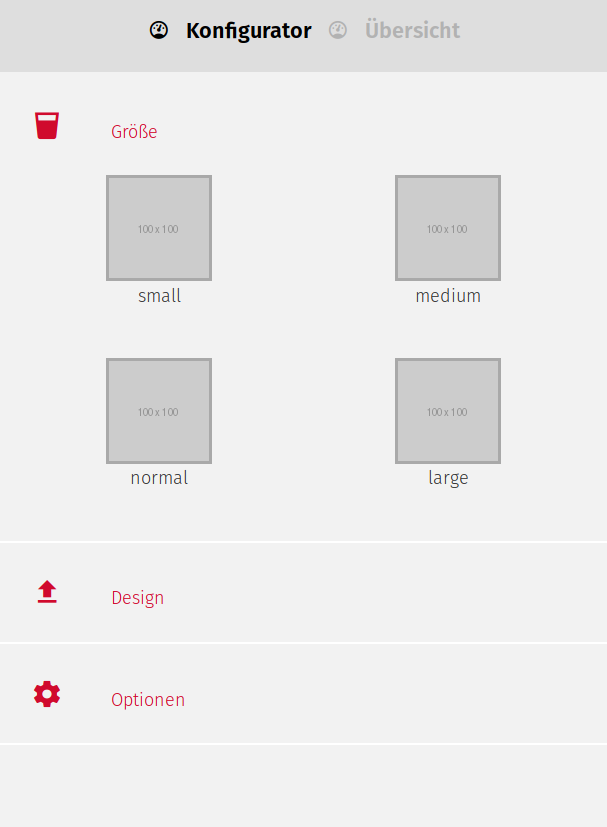
\epsfig{file = methodik/images/sidebar.png, width=8.0cm}}
	\caption[Sidebar des Konfigurators]{\textit{Sidebar der Angular-Anwendung}}
	\label{fig:sidebar}
\end{figure}


Zusätzlch hat die SidebarComponent auch noch eigene nicht geteilte Kindskompontenten. Das Konfigurationsmenü besteht aus Größe, Design-Upload und Optionen. Diese drei sind ebenfalls als Menü umgesetzt. Es handelt sich hier wieder um eine Bootstrap Komponente, das Accordion, welches ein aufklappbares Menü ist (\textit{Collapse})\footnote{https://getbootstrap.com/docs/4.0/components/collapse}. Die einzelnen Punkte sind hier auch wieder eigenständige Komponenten die als Kindskomponenten in der \textit{SidebarComponent} verwendet werden. Allerdings sind diese Komponenten weniger komplex. Hier sind alle Menüpunkte unterschiedlich aufgebaut, weshalb es 3 verschiedene Komponenten gibt. Das Accordion wird wie in der Dokumentation von Bootstrap verwendet. Wie das ganze am Ende aussieht kann man auch in Abbildung \ref{fig:sidebar} sehen. Die Komponenten \texttt{<gc-size>}, \texttt{<gc-upload>}, und \texttt{<gc-options>} sind dann sozusagen der Content. Die \textit{SizeComponent} und \textit{OptionsComponent} sind einfache \texttt{html}-Snippets. Die \textit{UploadComponent} ist wegen dem Upload-Vorgang des Designs etwas komplexer und wird später noch genauer beschrieben.
%
\section{3D Szene mit Model}
\label{sec:umsetzung}
%
\paragraph{Szene erstellen}Die \textit{SceneComponent} wurde schon angelegt. Nun muss noch die Funktionalität programmiert werden. In unserem Template ist alles was wir brauchen ein \texttt{<canvas>}-Element, \textbf{(ElementRef als Service erwähnen) }in dem dann später die ganze 3D Szene dargestellt wird. Zum Erstellen der 3D Szene und dem Laden der 3D-Models wird ein Service verwendet. Dieser Angular Baustein kann auch über die CLI angelegt werden. Der Service hat nun eine \texttt{createScene()} Funktion, die eine Scene mit Belichtung und Kamera erzeugt. Ihr wird als Parameter das \texttt{<canvas>}-Element übergeben. Für den Konfigurator wurden verschiedene Belichtungen verwendet, die ein optimales Licht erzeugen. Dabei handelt es sich um ein \textit{AmbientLight}, \textit{KeyLight}, \textit{FillLight} und \textit{BackLight}. Die Kamera hat verschiedene Werte zugewiesen bekommen, damit sie in der richtigen Perspektive den Becher später darstellt.
%
\paragraph{Model laden} Nun fehlt es noch an Leben in der Szene. Als 3D Model werden testweise Becher verwendet, die in etwa den späteren Mehrwegbechern entsprechen. Die 3D Models sind einfach \texttt{.obj}-Dateien, die aus 3D Programmen exportiert werden können. Mithilfe des \textit{OBJ-Loaders} kann man nun die Datei in die Szene laden. Jedoch stößt man da schnell auf das Problem, das die Loader nicht standardmäßig implementiert sind. Abhilfe schafft hier das \textit{npm}-Module \textit{full-three}\footnote{https://www.npmjs.com/package/three-full}. Es beeinhaltet die komplette Three.js Bibliothek mit allen Beispielen und Loadern. Nachdem also die Szene mit Kamera und Belichtung steht, wird die \texttt{.obj}-Datei geladen.
%
\begin{lstlisting}
const loader = new THREE.OBJLoader();
loader.load('assets/model/test.obj', this.onModelLoadingCompleted);
\end{lstlisting}
%
In der Funktion \texttt{onModelLoadingCompleted} wird dann der Renderer ausgeführt, die das Model zur Szene hinzufügt und anschließend alles rendert. Jetzt ist die 3D Ansicht schon mal mit Leben gefüllt, der nackte Becher angezeigt wird (siehe Abbildung \ref{fig:3dmodel}).
\begin{figure}[h]
	\centering
	{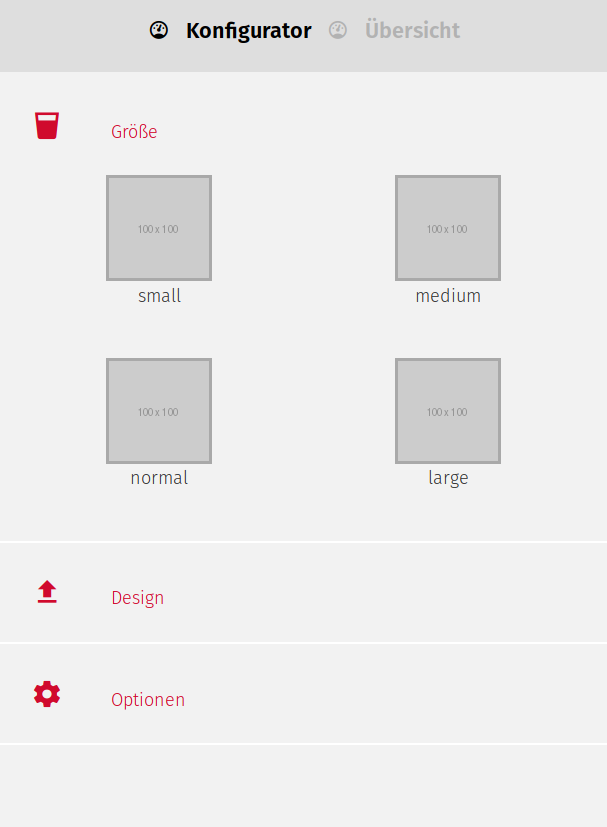
\epsfig{file = methodik/images/sidebar.png, width=8.0cm}}
	\caption[Komponentendiagramm]{\textit{Sidebar der Angular-Anwendung}}
	\label{fig:3dmodel}
\end{figure}
\paragraph{Auswahl der Größe}
Unter dem Menüpunkt \textit{\glqq Größe\grqq} soll der Benutzer eine der vier Größen wählen. Standardmäßig ist von Beginn an der 0,2 Liter Becher gewählt und ist von Angfang an sichtbar. Wie genau der DataService funktioniert, wird später noch einmal genauer beleuchtet. Zunächst werden in der \texttt{<gc-size>}-Komponente die verschiedenen Auswahlmöglichkeiten dargestellt. Mit der \texttt{onClick}-Funktion \texttt{reloadModel()} wird dem \textit{SceneService} mitgeteilt, das der Benutzer eine Bechergröße gewählt hat. 
%
\begin{lstlisting}
this.scene.remove(currentModel);

const loader = new THREE.OBJLoader();
const file = 'assets/model/' + model + '.obj';
loader.load(file, this.onModelLoadingCompleted);

this.controls.update();
this.render();
\end{lstlisting}
%
In der Funktion wird als erstes das aktuelle Model entfernt. Danach wird geprüft, welche Größe der User ausgewählt hat und dementsprechend wird das neue Model geladen. Anschließend muss die Szene neu gerendert werden. 
\paragraph{Controlling}
Der Becher soll in 3D angezeigt werden und soll rotiert werden können. In Three.js wird dafür \textit{OrbitControl} verwendet. Diese Klasse liefert verschiedene Werte mit, die verschiedene Einstellungen ermöglichen. Beispielsweise kann man die Rotationsgeschwindigkeit einstellen. Wenn man den Becher im Extremwinkel betrachtet oder zu weit hineinzoomt, kann der Becher bzw. dessen Texture unscharf aussehen oder nicht realistisch dargestellt sein. Deshalb wird über die Controls auch ein maximaler Zoom und ein maximaler Betrachtungswinkel festgesetzt.
\paragraph{Responsive} Die Ansicht sollte auf allen Displaygrößen darstellbar sein. Dafür sorgt der \texttt{@HostListener}. Dieser macht nichts anderes als die Fenstergröße zu überprüfen und das \texttt{<canvas>}-Element anschließend an den Container anzupassen. Falls sich die Fenstergröße ändert, wird der Szene über die Funktion \texttt{getAspectRatio()} die aktuelle Größe übermittelt. Dann wird die Szene aktualisiert und neu gerendert. Damit ist verhindert, das zum Beispiel auf kleineren Geräten der Becher abgeschnitten dargestellt wird oder ähnliches.
%
\section{Design Rendering}
\label{sec:umsetzung}
%
Jetzt geht es um das Hauptproblem der Arbeit: Auf dem Becher muss das Design des Kunden gerendert werden. Zunächst wird zum Testen ein Design erstellt, so wie es der Kunde hochladen würde. Nach verschiedenen Test, das Design direkt auf den Becher als Textur zu rendern wurde eine besser Lösung gefunden. 
\paragraph{3D Zylinder}
Die Bibliothek Three.js kann Geometrien erzeugen. Das heißt, man muss kein 3D Model aus einer Datei laden, sondern kann im Code eine geometrische Form erzeugen. Genau das wird für das Design des Bechers genutzt. Der Becher hat die Form eines Zylinders. Innerhalb der \texttt{onModelLoadingCompleted}-Funktion wird nun eine \textit{CylinderBufferGeometry}\footnote{https://threejs.org/docs/\#api/en/geometries/CylinderBufferGeometry} erstellt. Im Grunde umhüllt das Design den Becher wie ein Aufkleber.
%
\begin{lstlisting}
const geometry = new THREE.CylinderBufferGeometry(<radiusOben>, <radiusUnten, <height>, <radialSegmente>, <heightSegmente>, <offenesEnde>, <lenght>);
\end{lstlisting}
%
Durch die Parameter ist es möglich, den Zylinder genau an die Maße des Bechers anzupassen. Er liegt ganz eng auf dem Becher, eben wie ein Aufkleber. Mit dem Parameter \texttt{<offenesEnde>} wird festgelegt, das der Cylinder hohl ist und \texttt{<lenght>} stellt sicher, das der Zylinder 360 Grad im den Becher dargestellt wird.\footnote{Um das zu erreichen setzt man einfach den Wert auf \textit{2*Pi }}. Die anderen Parameter beschreiben den Radius und die Höhe des Zylinders. Im \textit{ThreeService} sind die Parameter der \textit{CylinderBufferGeometry} in Variablen für jeden der vier Becher definiert. Bevor die Geometrie erstellt wird, muss nur das aktuelle Model geprüft werden .Dann müssen die passenden Zylinder-Parameter für die aktuelle Bechergröße geladen werden. Somit umhüllt der Zylinder immer den ganzen Becher, egal welche Bechergröße gewählt ist.\\
Jetzt kann das Design des Kunden als Texture auf den Zylinder gepackt werden. Das praktische ist, das sich das Design an die Maße des Zylinders anpasst. Wenn das Design in der richtigen Auflösung hochgeladen wurde, sieht es somit realistisch aus\footnote{Im Upload-Vorgang wird der Benutzer bei falscher Auflösung des Designs darauf hingewiesen (siehe Kapitel 5.9).}. Aufgrund der kubischen Form des Zylinders wird das Design minimal gestaucht, genau wie beim Druck.
\begin{figure}[h]
	\centering
	{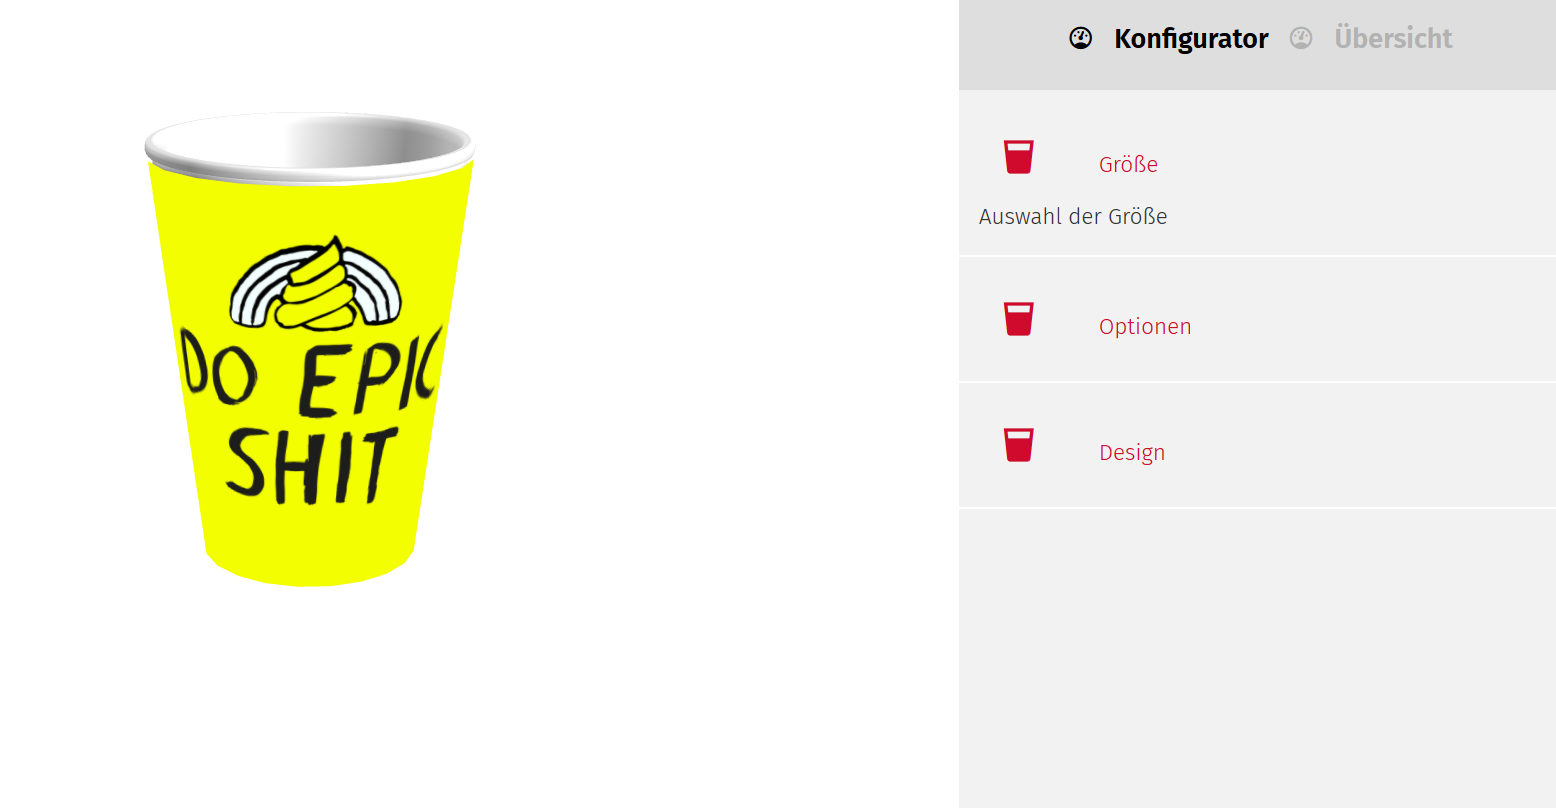
\epsfig{file = umsetzung/images/bechermitdesign.PNG, width=11.0cm}}
	\caption[Konfigurator mit designtem Becher]{\textit{Darstellung des Designs auf dem Becher mit Zylinder-Geometrie}}
	\label{fig:bechermitdesign}
\end{figure}
Da der Upload des Designs noch bis hierhin noch nicht implementiert ist, wird mit einem statischen Design gearbeitet. In Kapitel 5.9 wird sich diese Arbeit mit dem Upload-Vorgang beschäftigen. Solange allerdings kein Design als Texture hochgeladen wurde, wird der erstellte Zylinder in der Scene ausgeblendet. Es würde keinen Sinn machen einen blanken Zylinder um den Becher anzuzeigen. Die 3D Darstellung des Bechers mit Design funktioniert aber grundsätzlich schon, wie man in Abbildung \ref{fig:bechermitdesign} sehen kann.
%
\section{Mobile Umsetzung}
\label{sec:umsetzung}
%
Auf Tablets (in der Portraitansicht) ist es praktisch das Menü unterhalb der 3D Ansicht darzustellen. Das lässt sich ganz einfach mit den Column-Klassen von Bootstrap realisieren. Interessanter wird die Darstellung auf Smartphones.\\
Das Off-Canvas Menu ist vom Design nicht anders als die Desktop-Variante. Es wird lediglich verschoben. Das bedeutet, wenn ein Benutzer auf dem Smartphone den Konfigurator öffnet, sieht er zunächst nur den 3D Becher. Er kann dann das Off-Canvas-Menu über ein Hamburger-Menu-Button öffnen. Das ganze ist mit einer JavaScript Funktion realisiert, die einfach das Menü aus dem sichtbaren Bereich verschiebt und sie erst dann sichtbar werden lässt, wenn der Hamburger-Menu-Button gedrückt wird. Über \texttt{css} werden die SceneComponent sowie die SidebarComponent noch so angepasst, dass sie immer 100\% des Displays einnehmen. Außerdem werden die Schriftgrößen etwas größer gemacht.
Der Hamburger-Button ist ausschließlich auf Smartphones sichtbar. Wenn dieser geklickt wird, greift die Funktion \texttt{showsidebar()} bzw. \texttt{hideSidebar()}.
%
\begin{lstlisting}
document.getElementById("mySidenav").style.width = 100%;
\end{lstlisting}
%
Soll die Sidbar angezeigt werden, wird die Höhe auf \texttt{100\%} gesetzt. Soll sich geschlossen werden, wird die Breite auf \texttt{0} gesetzt. Damit ist eine sehr simple Lösung einer mobilen Sidebar implementiert.

Die 3D Szene ist, wie schon zuvor erwähnt, auch responsive. Die OrbitControls von Three.js liefern auch eine Kompatiblität für Touch-Eingaben mit. So kann auf mobilen Geräten der Becher via Touch rotiert werden.
%
\section{Daten-Service}
\label{sec:umsetzung}
%
Der DataService hat eine Aufgabe: Alle Daten des konfigurierten Bechers zu speichern und sie bei Anfrage einer Komponente wieder zurückzugeben. Dabei ist es wichtig das der Service nur einmal gestartet wird und die Daten global speichert. Hierbei handelt es sich also um ein Singelton. In Angular einen Service zu implementieren, ist recht unkompliziert. Analog zum \textit{SceneService} wird dieser auch über Angular CLI anzulegen. Anders als der \textit{SceneService}, welcher ausschließlich von der \textit{SceneComponent} verwendet wird, soll dieser global zugänglich sein. Dabei speichert er folgende Daten:
\begin{description}
	\item[selectedImage] Speichert die \texttt{png}-Datei, welche der User hochgelden hat
	\item[state] Hat den Wert \textit{true} wenn ein Bild ausgewählt wurde
	\item[designName] Speichert den Namen der Bilddatei
	\item[designSize] Speichert die Größe der Bilddatei
	\item[count] Speichert die Anzahl der Becher, die der Benutzer später drucken lassen möchte 
	\item[size] Speichert die vom Benutzer gewählte Bechergröße
	\item[stroke] Speichert, ob der Eichstrich mitgedruckt werden soll (Optionale Auswahl)
	\item[price] Zeigt den aktuellen Staffelpreis abhängig der gewählten Anzahl.
	\item[model] Speichert den Pfad zur \texttt{.obj}-Datei, welche gerendert werden soll
\end{description}
%
Die Eigenschaften \textit{designName}, \textit{count}, \textit{size}, \textit{stroke} und \textit{price} werden in der Tabelle \textit{OverviewComponent} als Bindung angezeigt. Somit ist immer die aktuelle Auswahl des Benutzers in der Tabelle. \\
Der \textit{DataService} ist somit ein Speicherort aller Informationen über den ausgewählten Becher und das verwendete Design. Es ist durchaus denkbar den Service später zu erweitern. Man könnte die Informationen auf einem Server sichern, sodass der User zu späteren Zeiten auf seine Konfiguration zurückgreifen kann. Angular bitet dafür eine einfache Realisierung über das \textit{HttpClientModule}.

Auch der \textit{SceneService} nutzt den \textit{DataService}. Zunächst bekommt der \textit{SceneService}, wie schon erwähnt, die Information, welche Größe gewählt wurde. Je nach dem welchen Wert \textit{size} dann hat, ändert sich das 3D-Model. Ähnlich verhält es sich mit dem Design, was als Textur auf dem Becher angezeigt werden soll. Im nächsten Abschnitt wird genauer beschrieben, wie ein Design hochgeladen werden kann, und welche Rolle der \textit{DataService} dort spielt.
%
\section{Upload-Vorgang}
\label{sec:umsetzung}
%
Angenommen ein Benutzer hat sich für eine Größe entschieden und möchte nun sein Design auswählen. In der Sidebar kann über einen Button die \textit{UploadComponent} geöffnet werden. Der User wird hier auch noch einmal darauf hingewiesen, die Druckvorgaben zu beachten.
\paragraph{Route zum Upload}
An dieser Stelle der Anwendung wird das \textit{Routing} verwendet. Normalerweise befinden wir uns in dem Konfigurator unter dem root-Pfad. Beim Upload ändert sich der Pfad zu \texttt{localhost/upload}. Unter dieser Route ist definiert, das die \textit{UploadComponent} angezeigt werden soll und nicht die \textit{SidebarComponent}. Hier kann der Benutzer jetzt sein Design auswählen (siehe Abbildung).
%
\begin{figure}[h]
	\centering
	{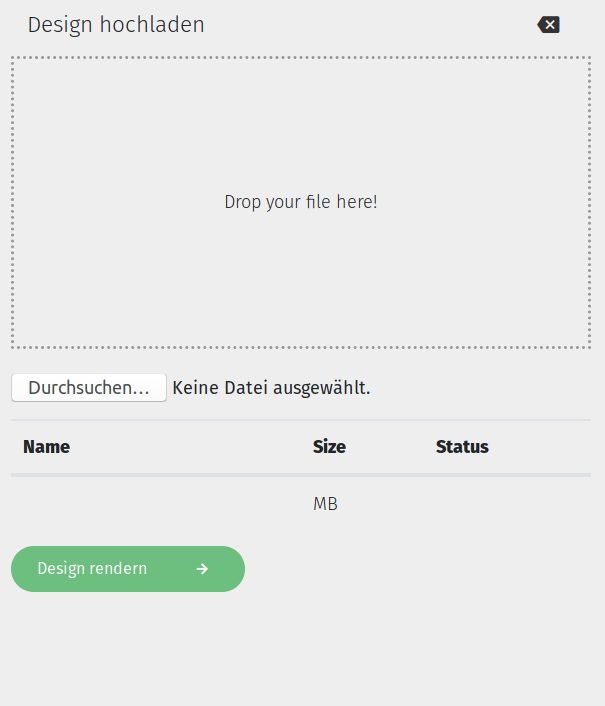
\epsfig{file = umsetzung/images/uploadcomponent.png, width=8.0cm}}
	\caption[UploadComponent des Konfigurators]{\textit{Upload-Komponente der Angular-Anwendung zum auswählen des Designs}}
	\label{fig:sidebar}
\end{figure}
%
Eigentlich ist der Begriff \glqq Upload \grqq nicht ganz zutreffend, da das Design nicht wirklich auf einen Server hochgeladen wird, sondern nur in dem \textit{DataService} gespeichert wird. Trotzdem ist klar, was die Funktion dieser Komponente ist. Der Benutzer hat zwei Möglichkeiten sein Design auszuwählen.
%
\paragraph{Drag \& Drop oder Select}
Eine bekannte Methode um Dateien hochzuladen ist die Drag \& Drop Methode. Man muss einfach die Datei in den dafür vorgesehenen Bereich ziehen und die Datei wird erkannt. Die zweite Möglichkeit ist es ganz klassisch über ein Input-Feld eine Datei aus dem Verzeichnis auszuwählen. Egal, für welche Methode der Benutzer sich entscheidet, passiert im Grunde das selbe. Ein Unterschied besteht darin, das verschiedene Eregnisse gebunden werden. Bei der klassischen Input-Feld Variante wird über das Event \textit{Change} überprüft, ob eine Datei ausgewählt wurde. Bei der Drag \& Drop Variante wird das Event \textit{drop} verwendet. Außerdem wird zusätzlich \texttt{dragover} und \texttt{dragleave} ausgeführt, wenn eine Datei in die Dropzone gezogen wird oder hinausgezogen wird. Für eine bessere Usability verändern sie die Farbe des Rahmens. Somit bekommt der User ein Feedback, wenn er seine Datei an die richtige Stelle gezogen hat.


In der \textit{UploadComponent} sind beide Upload-Vorgänge mit der Direktiven umgesetzt. In Diesen sind Dekoratoren implementiert, welche die eben erwähnten  Ereignisse über \texttt{@Hostlistener} binden. Für den Upload-Vorgang in diesem Konfigurator wird ein benutzerdefiniertes Ereignis benötigt. Um das zu erstellen verwendet man das \texttt{EventEmiter}-Objekt.
%
\begin{lstlisting}
private filesChangeEmiter: EventEmitter<File> = new EventEmitter();
\end{lstlisting}
%
Zusätzlich muss der Typ der Objekte explizit festgelegt werden. In diesem Fall wird ein \texttt{File}(einfache Datei) emittiert, jedes Mal, wenn der Benutzer eine Datei ausgewählt hat. Da der User nur ein Bild hochladen darf, ist dies nicht als Array implementiert. Nun können wir den \textit{EventEmiter} in \textit{@HostListener} verwenden. Es muss aber noch das Ereignis mit der übergeordneten HTML-Komponente gebunden werden. Dazu benötigt man den \textit{@Output} Dekorator für den \textit{EventEmiter}. Auf diese Weise ist es möglich zu überprüfen, ob sich die ausgewählte Datei geändert hat.
%
\begin{lstlisting}
<div gcDragDrop (filesChangeEmiter)="onFilesChange($event)">
\end{lstlisting}
%
Wie man im Beispiel sieht, wird jedes Mal, wenn eine Datei in die Drop-Zone geschoben wird, die Funktion \texttt{onFilesChange(\$event)} ausgeführt. Der Parameter \texttt{\$event} ist immer ausgewählte Datei. Die Methode kann jetzt mit diesem File arbeiten.\\

In der \textit{UploadCompontent} und auch an anderen Stellen der Anwendung soll der Dateiname und die Größe der Datei ausgegeben werden. Es ist nun möglich aus der übergebenen Datei beides auszulesen und in dem \textit{DataService} zu speichern. Nun muss noch die \texttt{reloadTexture()}-Funktion ausgeführt werden und die Datei übergeben werden. In Three.js werden Texturen mit dem TextureLoader geladen bzw. gemappt. Anschließend kann man sie zur Szene hinzufügen. Allerdings kann der Loader nur URLs oder Base64-Objekte entgegen nehmen. Auf den Pfad des Bildes können wir aus Sicherheitsgründen nicht zugreifen. Deshalb muss das File-Objekt in ein Base64-Objekt konvertiert werden, bevor man die Textur laden kann. Das konvertierte Objekt wird dann in \texttt{selectedImage} im \textit{DataService} gespeichert.
%
\begin{lstlisting}
this.getBase64(file).then(
	data => this.DataServ.selectedImage = data
);
\end{lstlisting}
%
Ist nun eine gültige \texttt{.png}-Datei ausgewählt worden, wird wie in Abbildung zu sehen Name und Dateigröße angezeigt. Jetzt ist auch der \textit{Design rendern}Button aktiv und das Design kann mit der \textit{reloadTexture}-Funktion gerendert werden.

\paragraph{reloadTexture}
Im Grunde ist diese Funktion nahezu identisch zu \texttt{reloadModel()}-Funktion. Ein Teil der Funktion ist schon bekannt. Wir haben schon gesehen wie diese Funktion den Zylinder für das Design um den Becher erstellt. Als Erstes löscht die Funktion eine Texture, die eventuell schon zuvor gerendert wurde. Nun bekommt die Funktion das Design des Users als Parameter übergeben und kann es als Texture gemappt werden.
%
\begin{lstlisting}[caption={TextureLoader Umsetzung},label=lst:texture]
const loader = new THREE.TextureLoader();
const material = new THREE.MeshBasicMaterial();
material.map = loader.load(image);
\end{lstlisting}
%
Um das ganze abzuschließend wird nun noch die Textur mit der Geometrie zusammengeführt und schließlich zu Szene hinzugefügt. Nachdem dann die Szene neu gerendert wurde, sollte das Design des Benutzers richtig auf dem Becher angezeigt werden.\\

Damit ist die Realisierung abgeschlossen. Die Funktionen wurden weitesgehend alle implementiert und müssen jetzt noch geprüft werden.